\chapter{Paying Off the Debt}
\label{chapter:refactoring}
In Chapter \ref{chapter:problem-description}, the extraordinary amounts of technical debt Tribler has accumulated over the past decade has been highlighted. We presented the architectural evolution from a historical perspective and proposed a new robust and future-proof architecture in Chapter \ref{chapter:architecture}. The top-level components of this new architecture, the GUI and RESTful API to communicate between the user interface and libtribler, have been implemented and discussed in \ref{chapter:towards-new-architecture}. We did however not focus yet on the libtribler component, which will can be considered as the core of the Tribler platform. Shaping libtribler to fit in the proposed architecture of Figure \ref{fig:tribler7}, requires some invasive refactoring efforts. Since this might be the most important component in our system, we will investigate libtribler in more detail and determine how we can identify and pay off the accumulated technical debt in the core. A summary of the re-engineering efforts conducted during this thesis work is displayed in Table \ref{table:refactoring-summary}.\\

\begin{table}[h!]
	\centering
	\begin{tabular}{|l|l|}
		\hline
		\textbf{Lines modified} & 765 \\ \hline
		\textbf{Lines added} & 12.429 \\ \hline
		\textbf{Lines deleted (without old GUI)} & 12.581 \\ \hline
		\textbf{Lines deleted (with old GUI)} & 25.010 \\ \hline
	\end{tabular}
	\caption{A summary of refactoring efforts as conducted during this thesis work, excluding the work on the new GUI.}
	\label{table:refactoring-summary}
\end{table}

Roughly, we can identify five different types of technical debt\cite{seaman2011measuring}: \emph{code debt}, \emph{testing debt}, \emph{infrastructure debt}, \emph{architectural debt} and \emph{documentation debt}. Tribler contains symptoms for every of the summarized types of technical debt.\\\\
We argue that refactoring in a dynamic typed language like Python is harder than when using a statically type language: information about naming errors  is not observed before runtime because of the lack of type information. This issue becomes apparent when for instance trying to rename a variable using a Python Integrated Development Environment (IDE): the application logic might miss various occurrences when performing the renaming operation and we become aware of this issue when either running Tribler itself or when executing the test suite. This shows the importance of having a solid, extensive test suite before we start to refactor major components in the system and we started with creating improvements to create a solid foundation for our refactoring efforts. Improving the test suite first has an additional advantage: by studying the test code, we can familiarize ourselves with the code base and review of the test code may help to us to understand the structure and detect code smells in the production code\cite{van2002video}.\\\\

%\section{Software Ageing}
%We start the discussing with introducing and discussing the term \emph{software ageing}, which we think is a phenomena that is particular visible in Tribler and that helps us to find root causes of the introduction of technical debt. Software ageing is a problem in a society that is dependent on all kinds of software. The term has been coined by Dave Parnas in his talk about software ageing in 1994\cite{parnas1994software}. He points out two major reasons why software ageing is a problem. The first is the lack of movement when software fails to meet the requirements of an always-changing environment: software that users perceived as state-of-the-art several decades ago, might now be considered as legacy software, mainly due to performance reasons. For instance, where a latency of several seconds when performing a remote search in Tribler might have been acceptable several years ago, users now expect system that responds to queries within a second.\\\\
%The second reason is in particular interesting since we think this is one of the most important reasons why Tribler has evolved to the complex, hard-to-understand architecture it is today and Parnas references to this phenomena as \emph{ignorant surgery}. Changes made by people who do not understand the original design concept almost always cause the structure of the program to degrade. This is especially true for the development process of Tribler which had many contributors who are making changes to specific parts of the architecture, often ignorant about the design concepts of the original authors of the code. Moreover, some developers might not be satisfied with the implemented design and decide to change the architecture to suit their own needs, possibly leading to an even more complex system.\\\\
%There are several approaches on how we can prevent or limit the process of software ageing. The first step towards the right direction, is to think about a design that is subject to change by applying the old slogan "design for change". This slogan is reflected in the flexibility requirement of the proposed architecture in Chapter \ref{chapter:architecture}. Various design principles are helpful to prepare a system for changes such as separation of concerns and using abstractions, however, many programmers fail to correctly apply these changes in software, either due to ignorance or recklessness. We should also note that it is notoriously hard to consider and think about possible changes in the future before starting to write code. This is in particular applicable to Tribler, where often a short-term research goal should be achieved: developers are writing a piece of software that they need for obtaining experimental results. New features are often the product of a publication or research project which are most likely not scheduled when designing an architecture of Tribler. In fact, it is not even certain that new features will be added after a specific release, since Tribler is not considered a complete commercial product that should meet customer's expectations (although we should try to achieve the highest level of user satisfaction).\\\\
%Design decisions taken during the development process are often not  documented. Developers fail to see the need for a proper documentation base and are proposing that the code is the documentation itself. However, this only works if you are following the structure they are using. Sometimes, it is more successful to communicate ideas on a higher-level, natural language that allows for less disambiguation. Tribler used to keep track of several design documents that describe the architecture, user interface decisions and research results, however, these documents are outdated and at the moment, there is no clear up-to-date description of the architecture. The lack of software artifacts will be discussed in more detail in Section \ref{sec:software-artifacts}.\\\\
%Parnas considers another option to limit software ageing: code reviews. For years, Tribler developers have created many new features which are not peer-reviewed by anyone, leading to a mix of different programming styles. Code reviews are an essential part in the software development process and should not be neglected.\\\\
%While prevention is a good medicine, we should define method that describe how we should deal with aged software. First of all, we can apply the methods we describe: change for design, code reviews and the construction of a proper documentation base. Modularisation of a system can be used to quicker identify components that are changing over time. When a product gets out of control, we should do a major restructuring of the product.

%\section{Influences of Python on software metrics}
%Tribler is written in: Python, an accessible, easy-to-learn language that is widely used in scientific applications. It is a high-level language, allowing one to express constructs with only a few lines of code. One of the most distinguishable properties of the language is that it is dynamically typed, which means that the type of a variable is not known at compile-time. This is in contrast to static typing, where this type is known to the compiler. The dynamic nature of the language has consequences on the way programmers are writing their code. A dangerous pitfall is that developers are making wrong assumptions about types of variables, leading to bugs that are only visible on runtime. Even then, it is not guaranteed that these kind of errors reveal themselves since they might be located inside a branch that is entered in a small amount of the application executions. Advantages of dynamic typing are apparent in testability since it is easier to mock objects during test execution.\\\\
%Dynamic typing also influences generated software metrics. While import graphs might give a good indicator of dependencies, they do not tell the whole story. In fact, there might be dependencies that are not visible in a generated import graph. These 'hidden' dependencies are often made between classes using the \emph{dependency injection} (DI) design pattern, a technique to not denote dependencies in the source code. For instance, if a class \emph{A} needs a particular service, this service is passed as parameter in a method call to \emph{A}. Dynamic typing makes it harder to capture such dependencies since almost no any information about types of attributes within a class can be determined at compile-time. The DI design pattern is very commonly used in Tribler and it is the preferred way to let components know about other components.

\section{Investigating the Debt}
It is hard to get accurate numbers on the amount of technical debt. When a decision to pay off technical debt is made, developers might run into unexpected situations that take longer than expected, especially if working with unfamiliar code. This makes estimations of the amount of work required unreliable. Several tools exist to monitor and estimate technical debt, the most prominent being CAST\footnote{http://www.castsoftware.com} (commercial) and SonarQube\footnote{https://sonarqube.com}\cite{falessi2015towards} (open source). In this Section, we will use SonarQube to track and identify the amount of technical debt in Tribler by setting up a SonarQube server to identify technical debt, bugs and vulnerabilities in the Tribler project. The reported results are summarized in Table \ref{table:sonarqube-metrics-summary}.\\

\begin{table}[h!]
	\centering
	\begin{tabular}{ l | l | l | l | l | l |}
		\cline{2-6} & \textbf{SLOC} & \textbf{Code smells} & \textbf{Bugs} & \textbf{Vulnerabilities} & \textbf{Estimated debt}\\ \hline
		\multicolumn{1}{ |l| }{wxPython GUI} & 20.080 & 2.139 & 11 & 0 & $\pm$ 21 days\\ \hline
		\multicolumn{1}{ |l| }{Qt GUI} & 2463 & 14 & 0 & 0 & $\pm$ 1 hour\\ \hline
		\multicolumn{1}{ |l| }{Tribler core (before refactor)} & 15.732 & 365 & 6 & 0 & $\pm$ 4 days\\ \hline
		\multicolumn{1}{ |l| }{Tribler core (after refactor)} & 15.700 & 117 & 0 & 0 & $\pm$ 2 days\\ \hline
	\end{tabular}
	\caption{The reported software metrics by SonarQube.}
	\label{table:sonarqube-metrics-summary}
\end{table}

The most interesting observation is that the wxPython GUI contains around five times more technical debt than the Tribler core and contains almost six times more code smells. To better investigate which files suffer from the most technical debt, SonarQube provides a bubble chart where the relation between the amount of technical debt, the number of code smells and the amount of code is visualized. For the wxPython GUI, this bubble chart is visible in Figure \ref{fig:technical-debt-wx-gui}. In this chart, the size of the bubble is correlated to the amount of code smells. The files suffering the most under technical debt are annotated with the file name. By taking Figure \ref{fig:wx-import-graph} as reference, we notice here that the files that contain the highest amounts of technical debt, are also the files with the most dependencies.\\

\begin{figure}[h!]
	\centering
	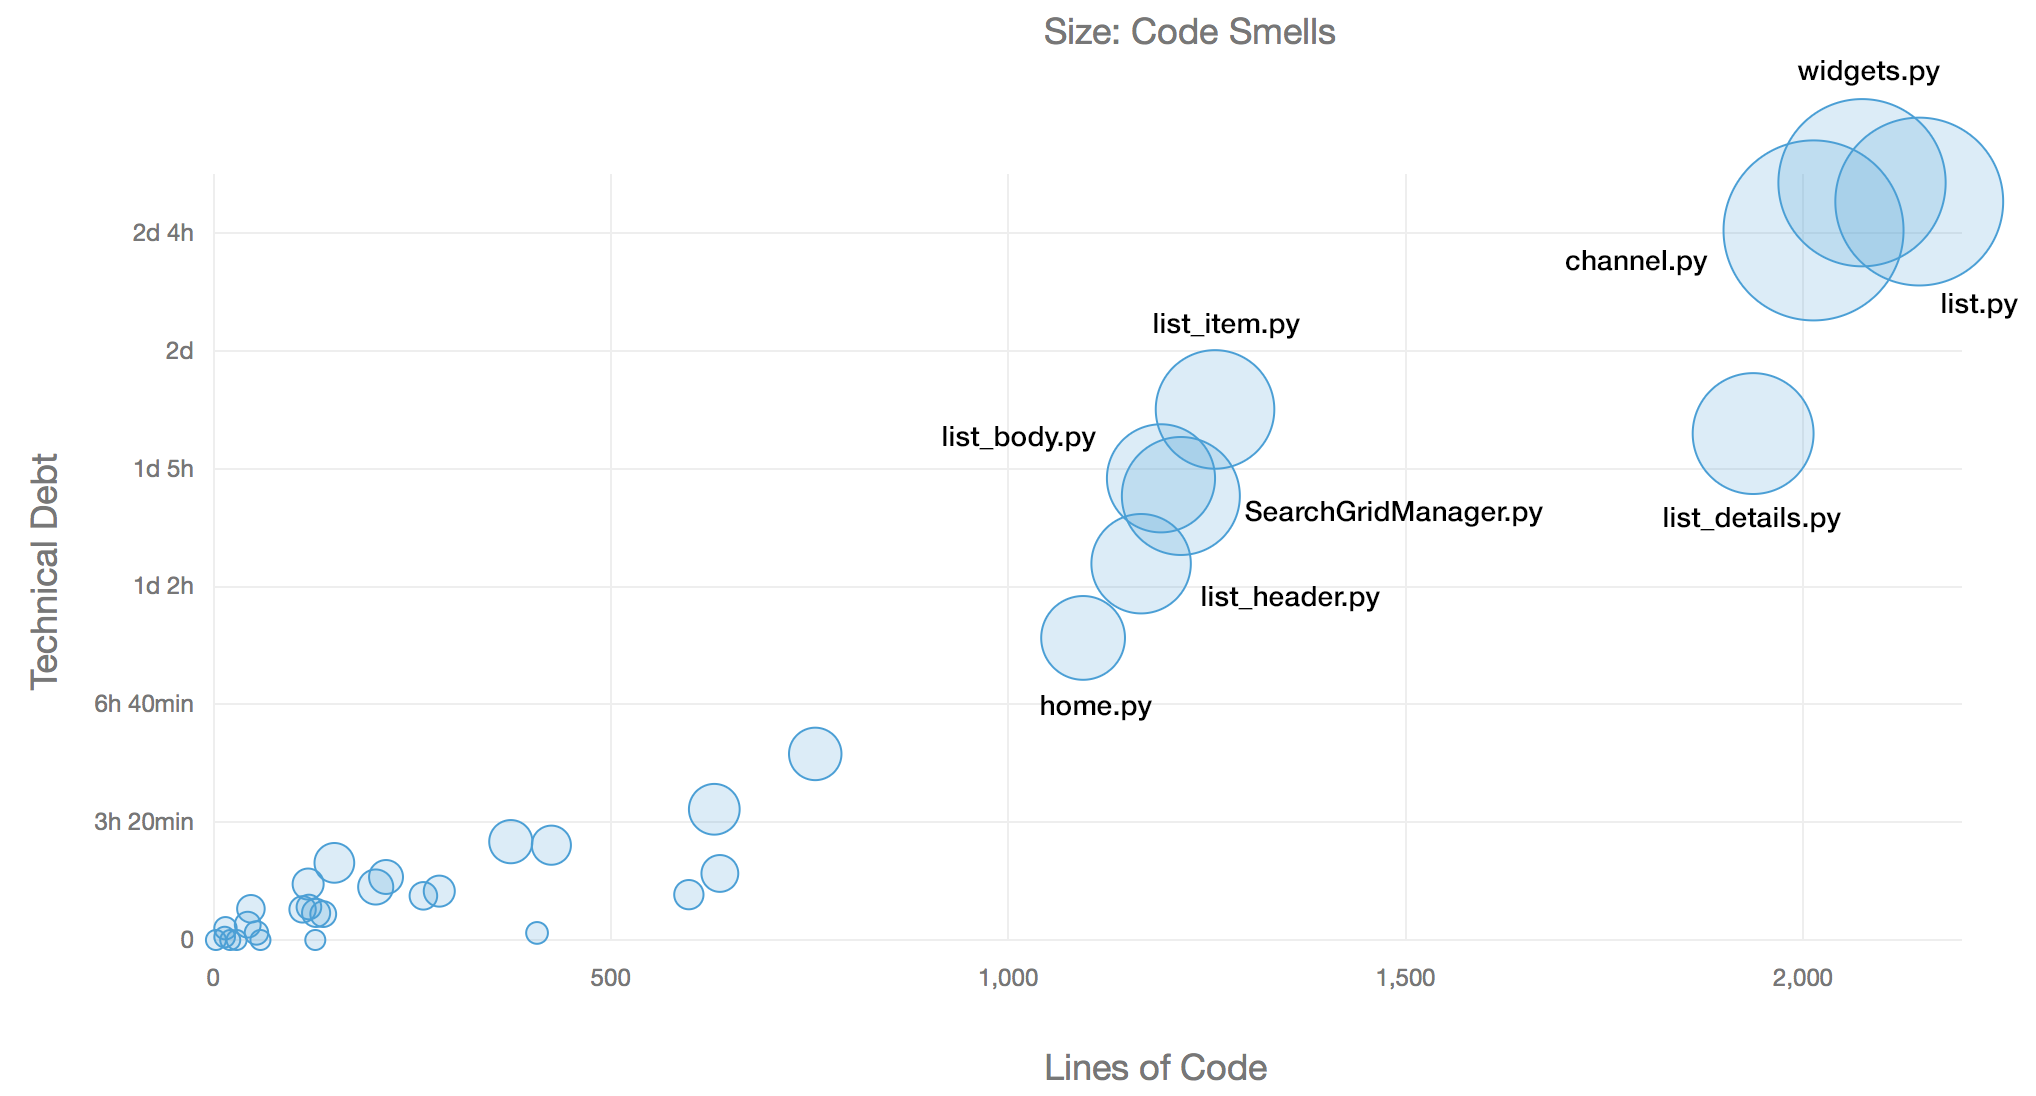
\includegraphics[width=1.0\columnwidth]{images/improving_qa/technical_debt_wx_gui}
	\caption{The amount of technical debt in the wxPython GUI reported by SonarQube.}
	\label{fig:technical-debt-wx-gui}
\end{figure}

\section{Code Debt}
We now turn our attention to the core of Tribler and present the bubble chart associated with the core package in Figure \ref{fig:technical-debt-core-before}. It is immediately evident that the \emph{SQLiteCacheDBHandler.py} file urgently needs refactoring. This file contains various utility classes to perform common database operation such as retrieval of specific channels and torrents. This file hosts the implementation of seven classes and our first effort consists of splitting this file into separate files where each file contains only one class definition.\\\\
However, we still identify many other files where technical debt is present in the form of code smells. We performed efforts to pay of this debt in the code base and will now summarize the most common identified code smells in the Tribler core package:
\begin{itemize}
	\item The cyclomatic complexity of various methods is too high, indicating that the procedure contains many independent linear execution paths. This negatively impacts the testability of this method since more distinct tests are necessary to guarantee an adequate coverage of the method. During this thesis, we reduced the complexity of several methods by splitting them into separate parts.
	\item We identified various methods that could be static. Static methods are meant to be relevant to all the instances of a class rather than to any specific instance. The usage of static methods is beneficial for performance and readability reasons. SonarQube recommends to use static methods where possible and we changed as much methods to static as possible.
	\item Naming conventions were not following during the development process and this is most notable in the inconsistency between the usage of \emph{CamelCase} practice and the usage of underscore notation. Since we wish to conform to the PEP8 styling guidelines\footnote{https://www.python.org/dev/peps/pep-0008/}, we should use the latter form. Part of efforts to pay off the identified code debt in the core includes work to rename of method, function, attribute and variable names to conform to the underscore notation. We should emphasize that some used libraries such as wxPython and PyQt are using the camelCase notation, leading to forced violation of this convention when overriding methods from this library.
\end{itemize}
The bubble chart of technical debt identified in the core after refactoring efforts described above is visible in Figure \ref{fig:technical-debt-core-before}. We emphasize the difference in scale on the vertical axis here compared to Figure \ref{fig:technical-debt-core-before}. The variance of the code debt has decreased significantly. Notice that the database handler definition files (that were originally located in the larger \emph{SQLiteCacheDBHandler.py} file) still contains some technical debt. However, there are many methods in these files that are unused when the new user interface will be deployed and could be removed at that point. Table \ref{table:sonarqube-metrics-summary} shows the statistics after our refactoring efforts. While we did not solve all code smells, we solve the most prominent occurrences of code debt and contributed to a more useful, maintainable and consistent code base.

\begin{figure}[h!]
	\centering
	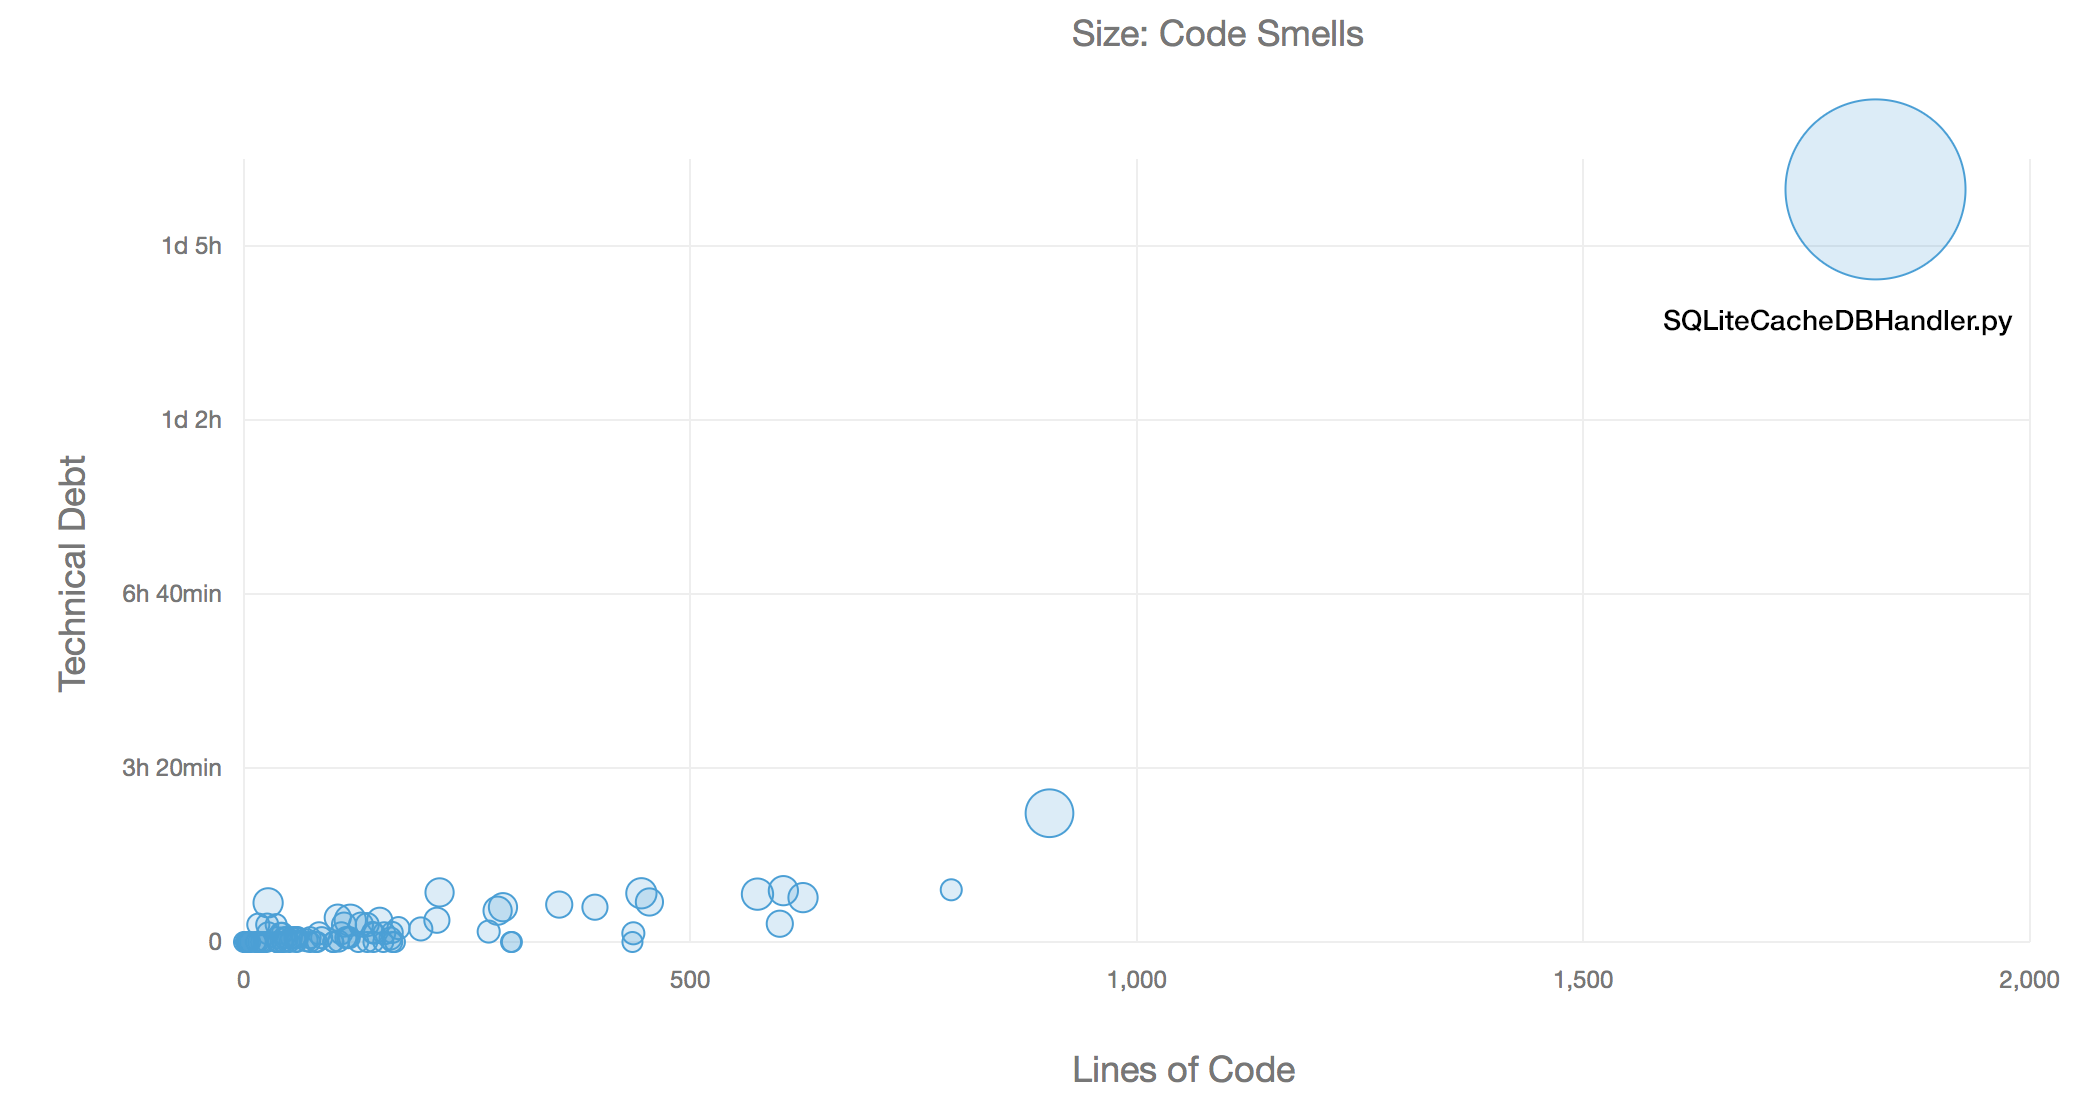
\includegraphics[width=1.0\columnwidth]{images/improving_qa/technical_debt_core_before}
	\caption{The amount of technical debt in the Tribler code reported by SonarQube before refactoring.}
	\label{fig:technical-debt-core-before}
\end{figure}

\begin{figure}[h!]
	\centering
	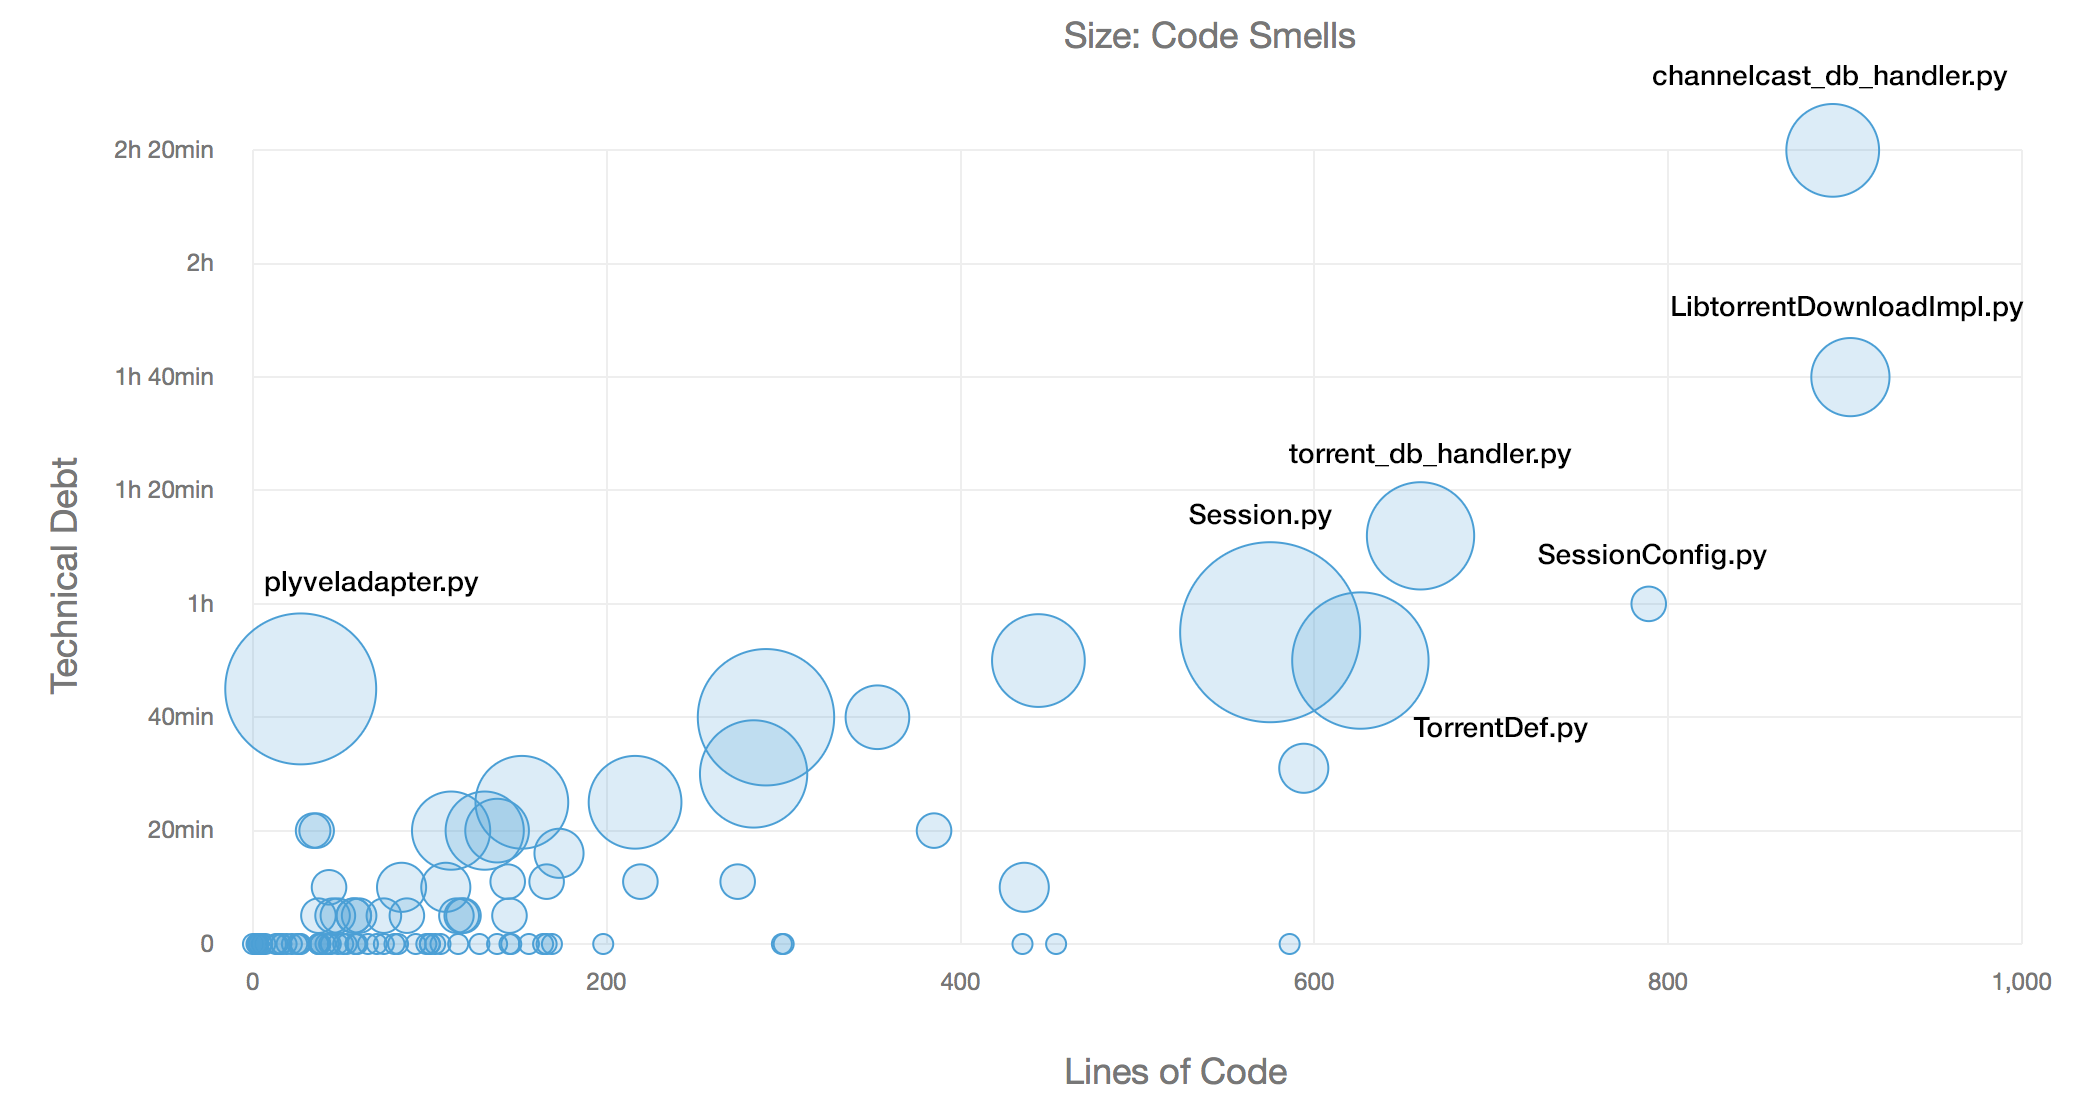
\includegraphics[width=1.0\columnwidth]{images/improving_qa/technical_debt_core_after}
	\caption{The amount of technical debt in the Tribler code reported by SonarQube after refactoring.}
	\label{fig:technical-debt-core-after}
\end{figure}

\section{Testing Debt}
The most fundamental way to verify a correct functioning of software is by having an well-designed and stable test suite. A solid test suite leads a to high quality bar, thus introducing a mechanism to keep the amount of technical debt under control\cite{sumit2016unittests}. As pointed out in Chapter \ref{chapter:problem-description}, the current test suite is plagued with unstable and non-functional tests. We will now focus on the performed work to strengthen and stabilize the test suite. A summary of the improvement of various metrics related to the test suite during this thesis is presented in Table \ref{table:test-suite-improvements}. Notice that the number of unit tests has dramatically increased, while the average execution time per test and the total duration of the tests has decreased.

\begin{table}[h!]
	\centering
	\begin{tabular}{ l | l | l | }
		\cline{2-3} & \textbf{November '15} & \textbf{July '16}\\ \hline
		\multicolumn{1}{ |l| }{Number of unit tests} & 80 & 676\\ \hline
		\multicolumn{1}{ |l| }{Number of assertions} & 117 & 1205\\ \hline
		\multicolumn{1}{ |l| }{Number of failed runs after 10 runs} & 2 & 0 \\ \hline
		\multicolumn{1}{ |l| }{TLC/PLC ratio} & 0.06 & 0.14 \\ \hline
		\multicolumn{1}{ |l| }{Total Linux test duration on Jenkins (sec)} & 448 (7 min. 28 sec.) & 350 (5 min. 50 sec.) \\ \hline
		\multicolumn{1}{ |l| }{Average execution time per test (sec)} & 18.90 & 0.85 \\ \hline
	\end{tabular}
	\caption{A summary of improvements to the test suite between November '15 and July '16.}
	\label{table:test-suite-improvements}
\end{table}

\subsection{Identifying Code Smells in the Tests}
As described in the work of van Deursen et al\cite{van2001refactoring}, there is a difference between refactoring test and production code in a sense that test code often has a characteristic set of code smells, originating from the way tests are structured. Before we start to make major modifications to the test suite, we present a list of code smells identified after a manual code review of the test suite of Tribler. This list is presented in Table \ref{table:tests-code-smells} where each code smell is described and a solution is proposed.\\

\begin{table}
	\begin{tabularx}{\textwidth}{|X|X|X|}
		\hline
		\textbf{Code smell} & \textbf{Description} & \textbf{Solution}\\ \hline
		Dependencies on external resources & Various tests are using external resources outside the test suite, leading to unpredictable and unstable tests. & Remove the dependency on the resource or make sure that the resource is locally available (see Chapter \ref{subsec:external-network-resources}). \\ \hline
		State leak & The state of a previous executed test is leaking to the next test, mostly notable due to delayed calls left in Twisted after completion of a test. & Make sure that any delayed call in Twisted is correctly removed when the test is completed. \\ \hline
		Too much responsibility & Many tests have multiple responsibilities, testing both parts of the user interface and core components in Tribler. & Make sure that each test is only verifying one small unit in the system. Also implement a separate bundle of tests for the user interface.\\ \hline
		Tests with a high execution time & There are some tests that are taking long to complete (sometimes over 30 seconds), negatively impacting productivity. This is an indication that the specific test has too much responsibilities. & Identify why the test takes long to complete and shorten the runtime i.e. by breaking the larger test into smaller parts. \\ \hline
		Unclear assertions & Tests that consists of multiple assertion statements often do not annotate this assertion well with a clear and meaningful description & Add an annotation with the cause of the failure if an assertion fails so developers can determine the problem quicker.\\ \hline
		Dependencies on a Tribler session & Some tests are starting a full Tribler session while only a small subset of the system is tested, leading to unpredictable circumstances. & Use mocking techniques to inject a mocked session or refactor the component so no session is required to test the component. \\ \hline
		Resource writing to source code directories & Various tests are writing resources to source code directories. They might accidentally end up in the Version Control System (VCS) if developers are not noticing these files. & Temporary resources produced by tests should always be written to a temporary directory that is cleaned up after test execution. \\ \hline
		Uncontrolled allocation of local network ports & Some tests that are running in parallel are claiming the same local network port, leading to test failures. & Reserve port ranges to individual parallel test runs or try to avoid the allocation of local ports. \\ \hline
		Timing issues & Some tests are checking for a condition after a fixed time interval. This interval is often based on intuition rather than empirical data. This is particularly dangerous when the test is dependent on external resources. & Refactor the test so the condition check is no longer necessary.\\ \hline
		No usage of code comments & There are no code comments that are explaining the purpose and expected output of the test. & Tests should be annotated with comments to explain the purpose of the test together with the expected in- and output. \\ \hline
		No directory structure in the tests package & There is no directory structure and a large amount of the tests are located inside the same directory. & Restructure the tests package and organise tests in different, logical named directories.\\ \hline
	\end{tabularx}
	\caption{Identified code smells in the test suite of Tribler as of November '15.}
	\label{table:tests-code-smells}
\end{table}

Table \ref{table:tests-code-smells} has been used as reference during the refactoring efforts of the test suite. We fixed most of the outlined code smells. Dependencies on external resources have been reduced to a minimum as explained in Subsection \ref{subsec:external-network-resources}. The efforts on increasing the stability of the tests is outlined in Subsection \ref{subsec:instability-tests}. During the refactoring process of tests, we placed clear assertions, added comments in the tests and got rid of managing Tribler sessions as much as possible.

\subsection{Improving Code Coverage}
Code coverage is defined as the percentage of SLOC that is covered by at least one test. Our continuous integration (CI) environment offers tools to track the code coverage over time. After each test suite execution, a comprehensive report with detailed information about the code coverage is generated. The reported metrics by this report are not accurate enough since some third-party libraries are included in the coverage report, such as the VLC bindings and \emph{pymdht}, a library to fetch peers from the DHT. We are not responsible for the code coverage of these libraries so we excluded them from the report.\\\\
A summary of improvements of the code coverage metric during the span of this thesis are displayed in Table \ref{table:code-coverage-table} where the SLOC and branch coverage is visible before and after this thesis work. Branch coverage is a metric that specifies how well conditional statements are covered and this metric includes the fact that a conditional is either resolved to true or false, possibly influencing the program execution path. In the ideal scenario, we wish to have tests that cover all conditional statements in the case they resolve to true and in the case they resolve to false so we cover all possible execution paths in the program. This objective gets significantly harder to achieve when dealing with code containing many nested conditional statements. The cyclomatic complexity as developed by McCabe in 1976\cite{mccabe1976complexity} is a quantitative measure of the number of linear independent paths through a program's source code. Any conditional written has a negative effect on the cyclomatic complexity. The branch coverage is usually lower than the SLOC since it is either hard to cover a specific branch or the missing branch might be considered as not unimportant. For instance, this might happen when we have a branch that only logs an event.\\\\
While at first sight it may look like the code coverage has not increased significantly, we should emphasize that the complete architecture of the tests have been overhauled. Refactoring of the test suite has consequences on the code coverage in other locations in the code base. To elaborate, the smaller unit tests are not starting the old user interface anymore, leading to a lower coverage in that module.\\\\
Improving the coverage has been done by writing small unit tests where we use mocked objects to control the system we are testing. The increase in the amount of unit tests is displayed in Figure \ref{fig:amount-of-tests-increase} where we annotated when this thesis has started. Using mocking is necessary since some components have many other dependencies that are hard to keep under control. Writing tests makes a developer more aware of the written code and it can be considered as a possibility to get familiar with an unknown code base. An additional advantage is that various bugs have been solved during the process of writing additional tests.\\

\begin{table}
	\begin{tabular}{ l | l | l | l | l | }
		\cline{2-5}
		& \multicolumn{2}{ | c | }{\textbf{November '15}} &
		\multicolumn{2}{ | c | }{\textbf{July '16} }\\
		\cline{2-5}
		& \emph{Lines coverage} & \emph{Branch coverage} & \emph{Lines coverage} & \emph{Branch coverage}\\ \hline
		\multicolumn{1}{|l|}{Tribler core} & 71,2\% & 58,1\% & 81,2\% & 67,3\%\\ \hline
		\multicolumn{1}{|l|}{REST API} & - & - & 99,4\% & 92,7\%\\ \hline
		\multicolumn{1}{|l|}{wxPython GUI} & 65,8\% & 42,7\% & - & -\\ \hline
		\multicolumn{1}{|l|}{Qt GUI} & - & - & 73,4\% & 50,4\%\\ \hline
	\end{tabular}
	\caption{The difference in code coverage between November '15 and July '16.}
	\label{table:code-coverage-table}
\end{table}

\begin{figure}[h!]
	\centering
	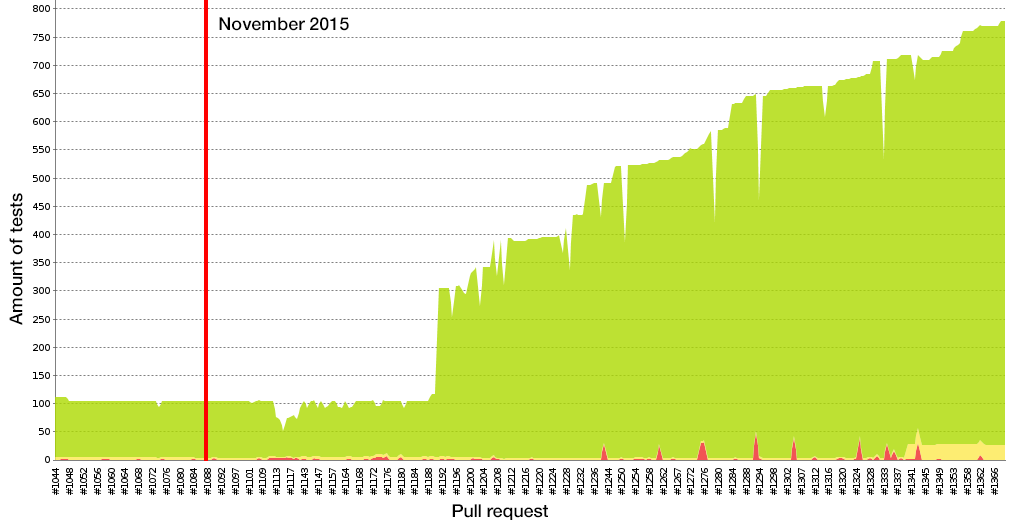
\includegraphics[width=0.8\columnwidth]{images/improving_qa/test_trend}
	\caption{The number of tests over time until July 2016 (November 2015 is annotated).}
	\label{fig:amount-of-tests-increase}
\end{figure}

In Figure \ref{fig:tests-ratio-tribler} the ratio between the number of code lines in the tests package and the amount of other code lines over time has been visualized. Together with the code coverage, this number can be a useful metric to developers. While one might argue that a high code coverage in conjunction with a low TLC/PLC ratio is a desired result, it indicates that the tests are not granular enough and are possibly performing many different operations. A low code coverage with a high TLC/PLC ratio indicates that there are some flaws in the tests, possibly that they are testing the wrong components of the system. In the case of Tribler when starting this work, the code coverage is reasonable but the TLC/PLC ratio is very low, indicating that most likely, the tests are not granular enough. This is in accordance with the discovered code smell that individual tests have too many responsibilities.\\\\
After writing additional unit tests, removal of the old user interface and addition of the new one, the new ratio is \emph{0.16} which means that there is roughly one line of test code for six lines of other source code in Tribler. Defining a good TLC/PLC ratio is dependent on the used programming language, development methodology and application structure. Discussion on the wiki of Ward Cunningham\cite{c2tlcratio} proposes an optional TLC/PLC ratio of 1:1, however, several other ratios have been proposed on the same page such as 2:1 and 5:1. In the work of van Deursen et al.\cite{van2001refactoring}, a ratio of 1:1 is proposed. Overall, the trend seems to be that the amount of test line code is around the same or a bit higher than the lines of production code. An important question is whether this proposed ratio is suitable for Tribler. Tribler differs from a commercial software engineering project in the sense that it is used for scientific research. When performing research, testing is considered a subordinate task and the main focus is gathering results that can be published. The difficulty here is that Tribler is distributed and used by over a million of users, requiring at least some form of quality assurance. We think an adequate TLC/PLC ratio for the Tribler project is between 1:2 and 1:4. With this ratio, we do not spent too much on writing tests while still maintaining a solid test base.\\\\
To make sure that the responsibility of code coverage is not neglected in future work on Tribler, an addition check for each pull request has been added that verifies that the code contributed in the respective pull request is covered by at least one test. While this check is not implemented by the author of this thesis, this is an effective way to keep the code coverage metric under control and to make developers more aware of the code coverage.

\subsection{Testing the GUI}
One of the issues identified in the tests package, was the lack of separation between tests that are testing the GUI and tests that are asserting core functionalities of Tribler. This is the main reasons that have led to big, individual tests in the old test suite. Since testing is an important aspect of this thesis work, constructing a solid test suite for the user interface code has been a prioritized task earlier in the development process.\\\\
User interface testing is a field of software engineering and is part of the application testing methodology. GUI testing can also be more involving than unit testing since a user interface might have many different operations and verification of the correct output of an action is often a non-trivial task. A common way of testing user interfaces is a Finite State Machine-based modelling where the user interface is modelled as a state machine that transitions when actions in the user interface are performed\cite{clarke1998automated}\cite{belli2001finite}. Another model to create a test script based on a genetic algorithms has been proposed by the work of Kasik et al\cite{kasik1996toward}. While these models might lead to good results when dealing with large application, consisting of many pages and transitions, we think they are unnecessary to utilize when testing the Qt user  interface at this point.\\\\
Testing the new Qt user interface uses the \emph{QTest} framework. This framework provides various tools to perform non-blocking waits in the tests and to simulate mouse clicks and keyboard actions. A sample of a test written with the \emph{QTest} framework is presented in Listing \ref{lst:qtest-sample}. This test has the following execution flow: after the interface is started, the test navigates to the home page, clicks on the \emph{channels} button in the header and waits for items to be loaded. During the test execution, two screenshots are taken, one when we are loading items and another one when the requested items are loaded and displayed.\\\\
Primitives to capture screenshots during test execution has already been implemented and used in the old test suite, using the rendering engine of wxPython. The Qt frameworks offers similar tools. Captured screenshots are saved as a \emph{jPEG} file and the name of the file is specified by the developer. In the sample presented in Listing \ref{lst:qtest-sample}, the exported screenshots are saved as \emph{screenshot\_home\_page\_channels\_loading.jpg} and \emph{screenshot\_home\_page\_channels.jpg} respectively. At the end of each test run, an image gallery is generated in our CI environment where the captured screenshots are archived and displayed in a grid. This allows developers to manually verify whether there are defects in the layout of the user interface. A part of the generated image gallery is displayed in Figure \ref{fig:jenkins-gallery}.\\

\begin{figure}[h!]
	\centering
	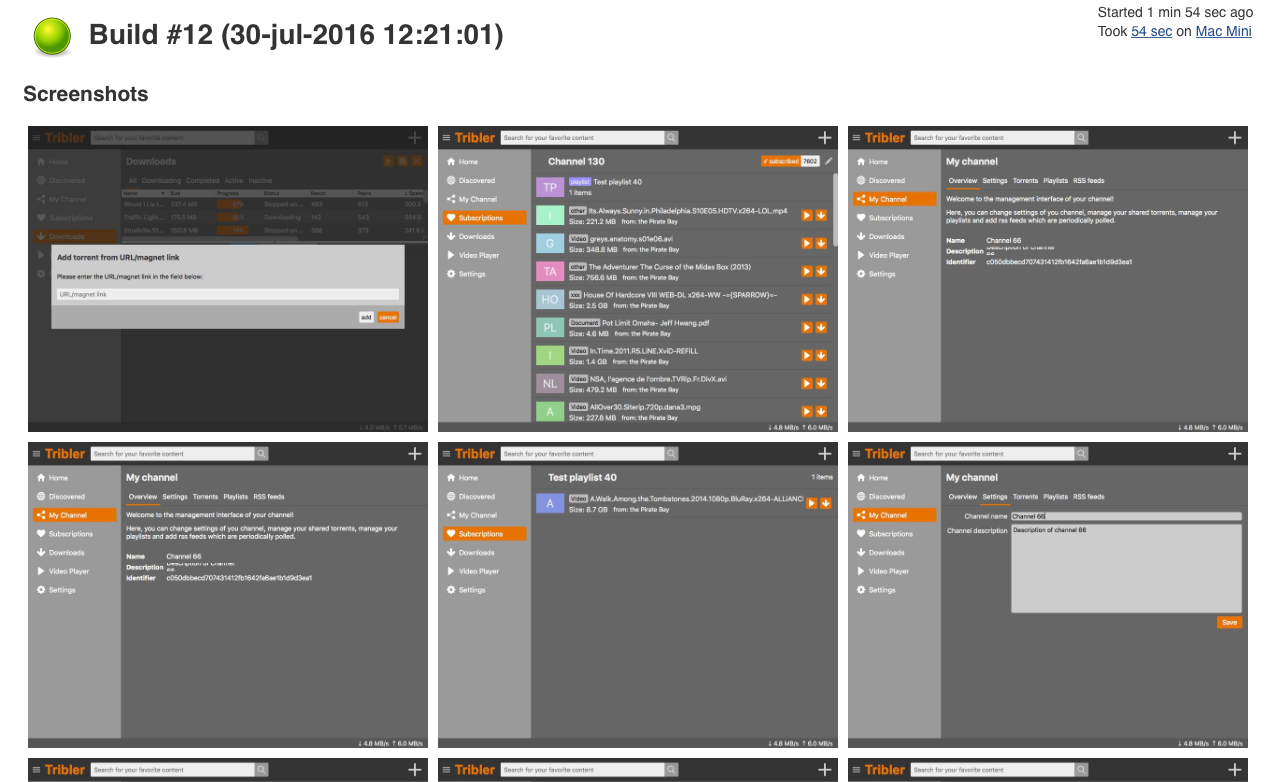
\includegraphics[width=1.0\columnwidth]{images/improving_qa/gallery_jenkins}
	\caption{The generated image gallery after executing of the user interface tests, generated by Jenkins.}
	\label{fig:jenkins-gallery}
\end{figure}

To avoid any dependency on core components of Tribler itself, we implemented a small piece of software that provides the same interface as the REST API implemented in Tribler. This 'fake' API is much simpler in nature and has a very simplistic in-memory data model. By utilizing this API, we are able to control API responses, significantly improving the predictability of the tests. The downside of this approach is that new endpoints have to be written twice, once in Tribler and once in this fake API.\\\\
A summary of several statistics related to these GUI tests is displayed in Table \ref{table:gui-tests-summary}. We note that the average execution time per test is higher than the time presented in Table \ref{table:test-suite-improvements}, however, during the tests we have various points where we have to wait for incoming data from the fake API provider.

\begin{lstlisting}[caption={A sample of a test that tests the new Qt Tribler GUI.},label={lst:qtest-sample}]
def test_home_page_channels(self):
	QTest.mouseClick(window.left_menu_button_home, Qt.LeftButton)
	QTest.mouseClick(window.home_tab_channels_button, Qt.LeftButton)
	self.screenshot(window, name="home_page_channels_loading")
	self.wait_for_home_page_table_populated()
	self.screenshot(window, name="home_page_channels")
\end{lstlisting}

\begin{table}[h!]
	\centering
	\begin{tabular}{|l|l|}
		\hline
		\textbf{Amount of unit tests} & 23 \\ \hline
		\textbf{Total execution time on MacOS} & 1 min. 4 sec. \\ \hline
		\textbf{Average execution time per test} & 2.8 sec.\\ \hline
	\end{tabular}
	\caption{A summary of statistics of the GUI tests.}
	\label{table:gui-tests-summary}
\end{table}

\subsection{External Network Resources}
\label{subsec:external-network-resources}
On of the identified code smells in Table \ref{table:tests-code-smells} is the dependencies on external resources, leading to unstable and unpredictable tests. To elaborate, the test suite contains various tests where external torrent files are fetched from the Internet, in particular, from the Ubuntu repository. While this repository guarantees a high availability, any downtime in this external resource leads to failing tests. The implemented solution for this flaw is to start up a local HTTP server that serves the torrent file. While this approach requires more code to manage this local server, it completely removes the dependency on the Ubuntu repository.\\\\
A similar solution has been applied to solve the dependency on seeders in the libtorrent network by setting up a local session that seeds a torrent. A small number of tests makes assumptions on the availability of torrent pieces. This dependency makes tests fail if the machine that runs the test has an unstable internet connection. Again, this approach requires code to properly start and shut down the seeder session, thus increasing complexity of the test suite. However, the implementation is reusable to an extend that developers of tests can reuse the implemented solution with only a few lines of code.\\\\
Unfortunately, there are various external dependencies left which are considered harder to refactor. A handful of tests are performing a remote keyword search, requiring various communities in Dispersy to be loaded. These tests are dependent on available peers in the respective community in order to ensure incoming search results. Due to time constraints, getting rid of this dependency is considered future work.

\subsection{Instability of Tests}
\label{subsec:instability-tests}
An unstable testing suite has a direct impact on the productivity of developers: when tests fails to reasons unrelated to the code that the developer contributed in a specific commit, developers have to execute the test suite again. One method to do this is by writing a comment on the Pull Request (PR) that says \emph{retest this please} on GitHub. Every retest operation is "wasting" several minutes since developers have to wait for the completion of test execution before they have the necessary feedback about the stability of their PR. This is a structural problems that Tribler developers are experiencing since the utilization of continuous integration.\\\\
To further investigate this structural problem, we estimate the total time developers had to wait for retests by writing a small script that uses the GitHub API to analyse every opened PR and count the amount of retests required before the PR is merged. Before we present the results, we should note that we might miss some occurrences since it is possible to remove comments on GitHub. In addition, some retests might be related to failures in the continuous integration environment and are not caused by flaws in the test suite. In total, we counted 2.045 retests in 1.481 pull requests, on average, 1.38 retests for each merged PR. If we use an optimistic estimation where an execution of the full test suite takes six minutes in total, we spent around 204 hours retesting pull requests. We argue that we can stabilize the test suite in much less time so we need no retests anymore. To demonstrate that we are dealing with a structural problem here since 2013, the number of retests over time has been displayed in Figure \ref{fig:retest-this-please-required}.\\

\begin{figure}[h!]
	\centering
	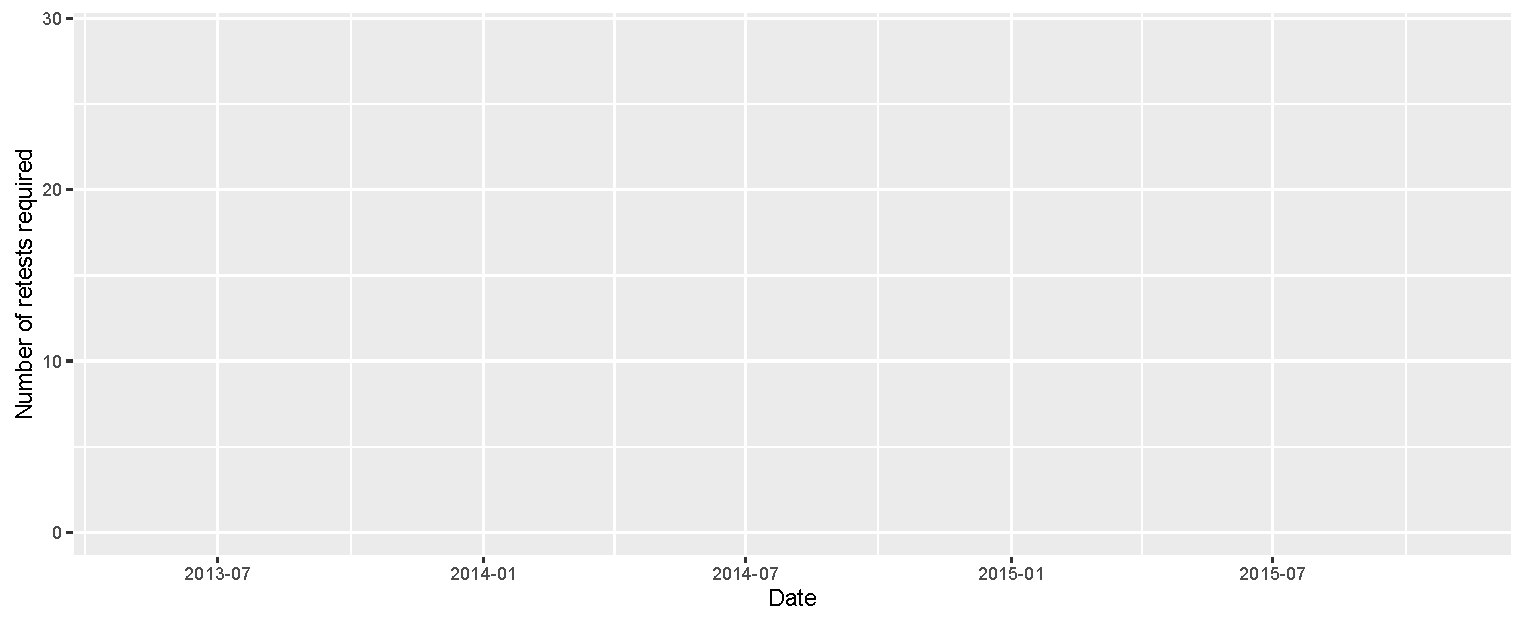
\includegraphics[width=1.0\columnwidth]{images/improving_qa/retests_required}
	\caption{The number of retests required in PRs over time.}
	\label{fig:retest-this-please-required}
\end{figure}

Essentially, we are dealing here with a special kind of technical debt. Developers prudently made the decision to postpone fixing of the problems in the test suite by retesting the PR until the tests suite succeeds. The incentives to spent some time to fix test errors are not apparent and often, developers do not feel that they are responsible for failing tests since it might have been caused by code written by other developers. This makes it attractive to ignore test failures.\\\\
Well-designed tests should only fail if some new code is breaking existing functionality. If no changes are presents, the tests should always succeed, regardless of how many times it is executed. Reducing dependencies on external resources is not sufficient to guarantee this desired property. The structural problem of the tests is that the system is infected a great amount of race conditions. Race conditions can be hard to spot since they often occur in a very specific runtime setting, making the debugging process of these kind of errors frustrating. In fact, it is very easy to deliberately introduce a race conditions that is not noticed after the code is merged into the main branch. A complex architecture is of direct influence on this phenomena and leads to more race conditions.\\\\
During this thesis, various race conditions have been detected and solved. One interesting observation is that some issues only occurred on a specific platform. We believe can be explained by differences in the implementation of underlying threading model across operating systems. The most common origin of the detected race conditions is addressed to delayed calls in Twisted. During the test execution, Tribler is started several times. If a developer leaves a delayed call behind when the shut down procedure has been completed, this delayed call might be executed in the wrong Tribler session, possibly leading to an inconsistent state of the system. Making sure Twisted is void of any delayed call is not straightforward: if one is not aware of scheduled calls in the system, the mistake is easily made.

\section{Infrastructure Debt}
Tribler makes use of the popular CI platform Jenkins. Jenkins allows developers to define jobs which can be executed manually or when pushing a commit on the code base. This CI platform is responsible for running the tests, packaging Tribler and running research-oriented experiments on the DAS5 supercomputer.\\\\
We noticed that the test suite is only executed in a Linux environment. Beller et al\cite{beller2016oops} conducted research on CI adoption and usage and it turned out that for some languages, it might benefit to run tests in different environment. We strongly agree with this vision and since Tribler is shipped for multiple platforms, we think it is of uppermost importance to run the unit tests in different environment. An addition argument for this is the presence of some platform-specific workarounds in Tribler. To make sure that these statements are covered by the tests, we must run the test suite in a specific environment. This will allow developers to detect defects on other platforms more earlier in the development process. By aggregating the generated coverage report on each platform, this multi-platform set up should have a (small) positive influence on the code coverage metric.\\\\
The set up of the testing environments on Windows and MacOS is straightforward: new slave nodes to specify the Windows and MacOS test runners have been created. The tests on MacOS are executed on a Mac Mini, late 2014 model with 4GB of DDR3 memory and an Intel Core I5 1.4 GHz processor. In order to run the tests on Windows, two virtual machines using Proxmox\footnote{https://www.proxmox.com}, a server virtualization management platform, have been created, both with 32-bit and 64-bit environments. After the utilization of these additional machines, the tests are executed on four platforms: Linux, Windows 32-bit, Windows 64-bit and MacOS. So far, both the MacOS and Windows test executers have completed over 2.700 test executions. Each test runner generates a coverage reports and these reports are merged in the final analysis step in the build pipeline.

\subsection{Future Improvements}
While this is certainly a step in the right direction, there are additional steps in the execution plan that could enhance the testing procedure. In Figure \ref{fig:jenkins-pipeline}, we present what we think is the ideal test execution plan, together with the various stages in this pipeline. The dashed boxes are jobs in the pipeline that are not implemented yet. The pipeline starts by the execution of the tests on multiple platforms where during these runs, the code coverage is being tracked. After this phase, the coverage reports are combined and the total difference with the upstream branch is determined. When the commit decreases the total code coverage, the job fails and the pipeline aborts. This negative result is visible on GitHub.\\

\begin{figure}[h!]
	\centering
	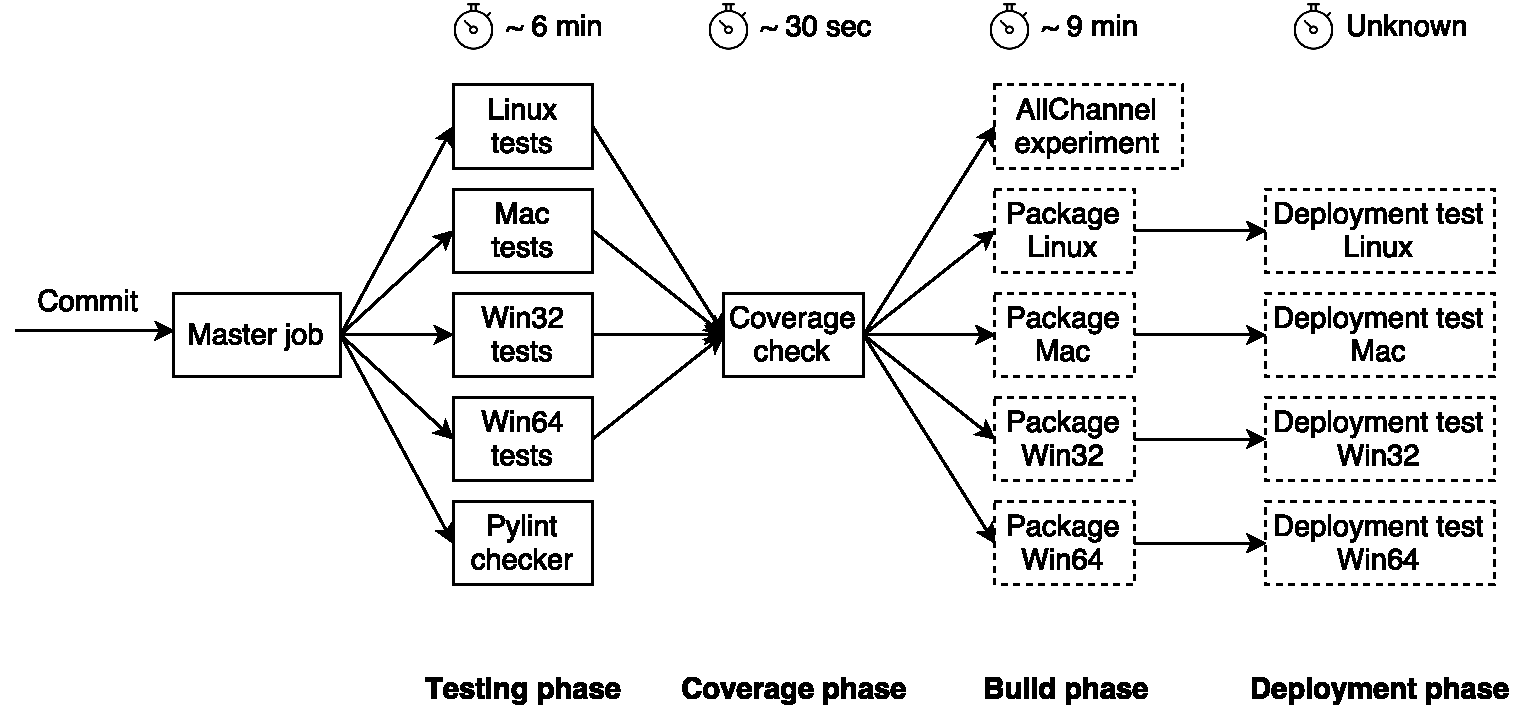
\includegraphics[width=0.9\columnwidth]{images/improving_qa/jenkins_pipeline}
	\caption{The desired test execution plan in our CI environment. Dashed boxes are not implemented yet.}
	\label{fig:jenkins-pipeline}
\end{figure}

A static Pylint checker to check for code style violations has been available for a long time, however this only gave insight in the total amount of Pylint errors in the whole code base and did not stimulate to actually fix errors in the committed code of a developer. While not implemented by the author of this thesis, the Pylint checker has been extended to fail if new violations are introduced in committed code. Additionally, a report is generated with an overview of the introduced violations, together with the relevant source code. This helps developers to get more aware of their code style and helps to realise a consistent code base. This check is executed in parallel with the tests to decrease the total time of the pipeline execution.\\\\
After the coverage phase has passed, the \emph{AllChannel} experiment should be performed. This experiment is executed on the DAS5 supercomputer and starts 1.000 Tribler clients that are synchronizing torrent and channel information with each other. When the experiment is completed, various graphs are generated, providing developers insights in the performance of their modified code when Tribler runs in a more large-scale setting. For instance, the experiment can highlight introduced issues in the message synchronization between peers in the network.\\\\
In parallel with the \emph{AllChannel} experiment, we should package Tribler for distribution to end-users. The purpose of this step is so we can execute deployment tests on various platforms to check whether Tribler works when distributed to end users. On Windows, an installer will be created that installs Tribler to the \emph{Program Files}. On MacOS, we create a \emph{DMG} file that contains an app bundle. On Linux, the required files are bundled in a \emph{deb} archive. All these packaging and deployment testing jobs can be executed in parallel to shorten the time of the testing pipeline.

\section{Architectural Debt}
Already indicated by Figure \ref{fig:wx-import-graph}, Tribler is plagued with many dependencies that are leading to a highly coupled system where it is hard to reuse individual components. We aim for a low coupling to increase testability of packages. This Section will focus on identification and removal of undesired dependencies between packages.

\begin{figure}[h!]
	\centering
	\begin{subfigure}{.5\textwidth}
		\centering
		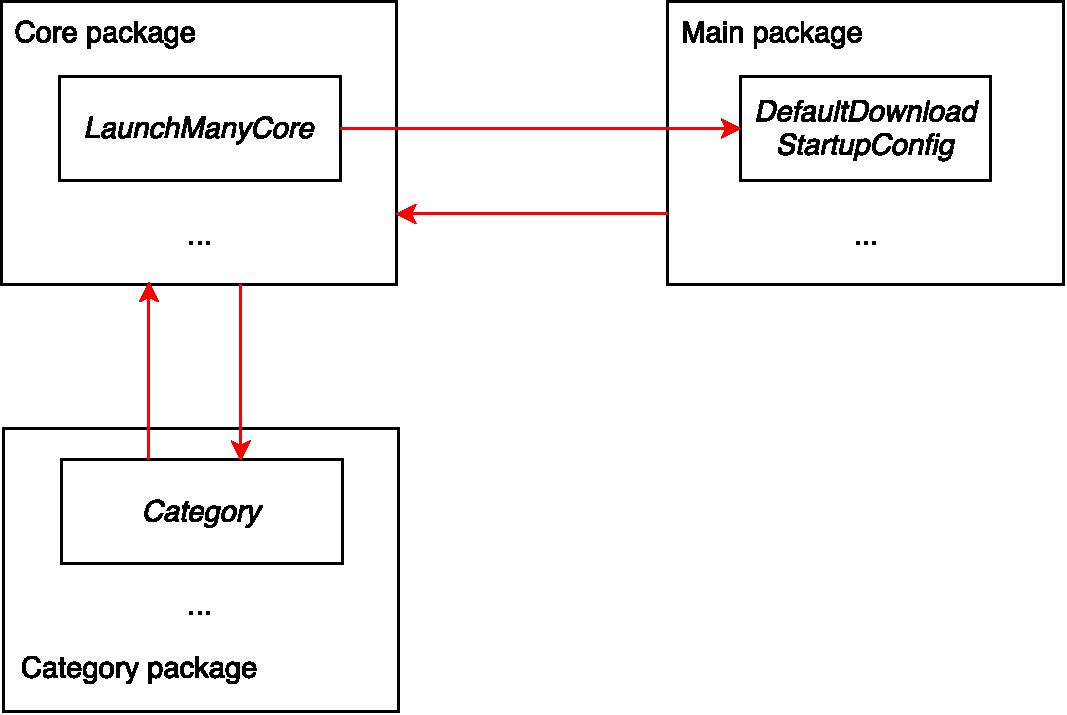
\includegraphics[width=0.9\linewidth]{images/improving_qa/cycle_tribler_package}
		\caption{Before refactoring}
		\label{fig:tribler-packages-refactoring-before}
	\end{subfigure}%
	\begin{subfigure}{.5\textwidth}
		\centering
		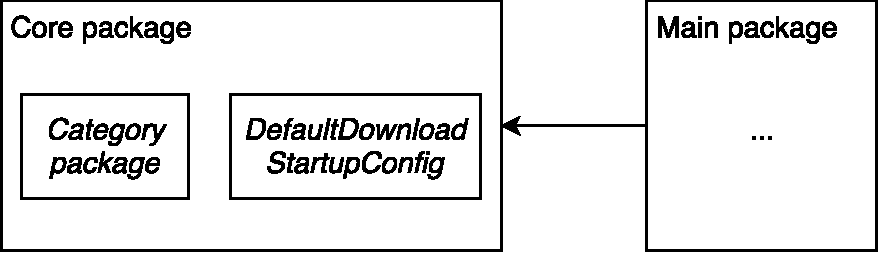
\includegraphics[width=0.9\linewidth]{images/improving_qa/cycle_tribler_package_after}
		\caption{After refactoring}
		\label{fig:tribler-packages-refactoring-after}
	\end{subfigure}
	\caption{The dependencies between Tribler modules at the highest level.}
	\label{fig:tribler-packages-refactor}
\end{figure}

\subsection{GUI and Core Dependencies}
\label{subsec:gui-core-packages}
As described in Chapter \ref{chapter:problem-description}, the source code for the user interface and Tribler core code is interleaved to a large extent and there is no clear separation between these components. There are various instances where we identified code present in the GUI code base that should be moved to the core and vice versa. To realise a clear separation between \emph{libtribler} and the user interface, we should make sure that we move code to the package where it belongs.\\\\
In the present code base, the \emph{Core} package is dependent on the user interface which is undesired: we are unable to utilize the Tribler core without the GUI code being present, leading to higher coupling. The exact dependency is visible in Figure \ref{fig:tribler-packages-refactoring-before} and is caused by the \emph{DefaultDownloadStartupConfig} class which is located in the \emph{globals.py} file, part of the GUI package. This class is responsible for providing default configuration options when a download is being started, in case the user did not override default options like the destination of the downloaded file and the amount of anonymous hops used. Since the superclass of \emph{DefaultDownloadStartupConfig}, \emph{DownloadStartupConfig}, is already located in the Tribler core, it makes sense to move the \emph{DefaultDownloadStartupConfig} class to the \emph{DownloadConfig.py} file, which already contains the \emph{DownloadStartupConfig} class. After we moved this class to the core and modified the references to point to the new location of the class, the core is completely independent of the user interface, displayed in Figure \ref{fig:tribler-packages-refactoring-after}.

\subsection{Category Package}
Referring to Figure \ref{fig:tribler-packages-refactor}, we note a cyclic import dependency between the \emph{Core} and \emph{Category} package. The \emph{Category} package hosts the source code to facilitate the family filter. Obviously, the family filter is used by the Tribler core, however, the family filter also has dependencies on classes inside the Tribler core, causing the cyclic import.\\\\
In the architecture proposed in Figure \ref{fig:tribler7}, we specified the family filter as a component of libtribler. We think that the best solution to solve this dependency, is to move the \emph{Category} package to the Core package so it's part of libtribler. This change is reflected in Figure \ref{fig:tribler-packages-refactoring-after}.

\subsection{Video Player}
We will now zoom in on the core package which contains some GUI-related code that should not be present in that package. The most obvious occurrence is attributed to management of the (embedded) video player in Tribler which is handled by the \emph{VideoPlayer} class in the \emph{Video} package. Figure \ref{fig:video-package-refactoring-before} shows the import graph of the  \emph{Video} package before refactoring. The \emph{VideoPlayer} class makes use of the VLC bindings for Python, however, in our design, the core does not need to have any dependency on VLC since managing the video player is a operation that should be performed on the user interface level. The \emph{LaunchManyCore} class contains code to initialize all components available in Tribler, including the \emph{VideoPlayer}. When initializing, this \emph{VideoPlayer} creates a \emph{VideoServer} that is responsible for the streaming capabilities of Tribler. The \emph{VLCWrapper} class contains various utility methods to work with raw VLC data such as the time position within a video.\\\\
We performed refactoring work within this package and removed the \emph{VideoServer} and \emph{VLCWrapper} classes. The composition of the \emph{Video} package after this operation is displayed in Figure \ref{fig:video-package-refactoring-after}. We modified the code such that the  \emph{LaunchManyCore} class starts a video server instead of a video player. We point out that there are some classes that are unused now, such as \emph{VideoUtility} and \emph{utils}: these classes contains some helper methods to retrieve thumbnail images from a video file and is considered legacy code. Due to time constraints, we are unable to implement these features in the new user interface so for now, we keep these files as reference for future development.

\begin{figure}
	\centering
	\begin{subfigure}{.5\textwidth}
		\centering
		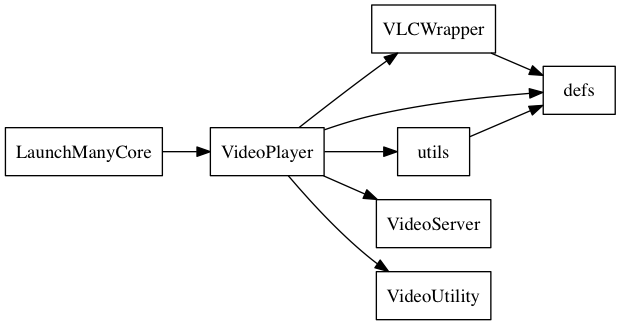
\includegraphics[width=.9\linewidth]{images/implementation/output_video_nov15}
		\caption{Before refactoring}
		\label{fig:video-package-refactoring-before}
	\end{subfigure}%
	\begin{subfigure}{.5\textwidth}
		\centering
		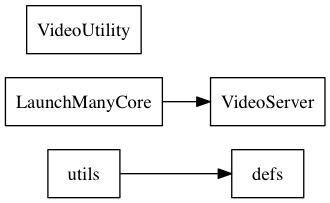
\includegraphics[width=.7\linewidth]{images/implementation/output_video_july16}
		\caption{After refactoring}
		\label{fig:video-package-refactoring-after}
	\end{subfigure}
	\caption{The import graph of the \emph{Video} package in the Tribler core before and after refactoring.}
	\label{fig:video-package-refactoring}
\end{figure}

%\section{Updating software dependencies}
%A cause of ageing software is the inability of developers to adopt to changing environment. This might be addressed to adoption of dependencies in the past, dependencies that are not maintained any more at a point in the future. Replacing these dependencies might be a non-trivial programming task, requiring the programmer to get familiar with both the interface of the old and new dependency.\\\\
%Tribler has a long list of dependencies, both in the code base and dependencies that are used for software packaging and testing. Keeping these dependencies on the latest version is often neglected or overlooked. Sometimes, this is not even possible, due to missing software in package managers such as \emph{yum}, the package manager used by CentOS or \emph{apt}, the package manager of Debian and Ubuntu. While this restriction holds for operating systems where we are not packaging dependencies, we have the freedom to package any dependency we want on Windows and MacOS so preferably, we often want to ship the latest, stable release of a dependency in our Tribler distribution.\\\\
%During this thesis, we updated several dependencies to newer versions, most notably \emph{libtorrent}. The code to handle the communication with this library (located in the \emph{Libtorrent} package) contained calls to deprecated functions in the \emph{libtorrent} library, functions that are not guaranteed to be maintained or compatible. We identified these calls as follows: first, a version of \emph{libtorrent} has been compiled without deprecated methods and assertions. Next, we manually ran Tribler and the test suite, observing any crash due to libtorrent. In total, this method yielded seven calls to deprecated methods that have been updated to call the correct function. Not only deprecated calls have been removed, we also fixed various assertions that were triggering due to incorrect assumptions made in the code. In order to remain backwards-compatible with older version of the libtorrent library (that some Ubuntu or Debian users might have installed on their system), some checks in the Tribler code base had to be implemented to check for the presence of a particular method in libtorrent.\\\\
%An additional outdated dependency in Tribler is \emph{py2exe}, used to create a Windows executable file out of the source code. \emph{py2exe} performs a static code analysis and determines code dependencies that should be bundled in the executable. Unfortunately, the library has not been updated since 2014 and requires a significant amount of code to make sure that everything works when Tribler is packaged and archived. We made attempts to replace \emph{py2exe} with the more mature, well-maintained \emph{PyInstaller} that also offers support for \emph{PyQt5}, the framework used for creation of the new interface. This library is not only easier to use, it also works across multiple platforms, allowing us to also drop the \emph{py2app} dependency which is used to distribute Tribler on MacOS. While not ready for deployment yet, a proof-of-concept has been created that successfully packages Tribler together with the new user interface into Windows and MacOS executable files. Further work should focus on the removal of \emph{py2exe} and \emph{py2app} in favour of \emph{PyInstaller}.

\section{Documentation Debt}
\label{sec:software-artifacts}
During the last ten years of development efforts on Tribler, the main focus of the project has been to deliver working code. The project has a severe lack of updated software artifacts, including documentation, code comments and architectural diagrams, leading to a huge amount of \emph{documentation debt}. Some of the conducted research was documented on the Tribler wiki\footnote{https://www.tribler.org/TitleIndex/}, however, this wiki contains many outdated pages and is not used or maintained anymore. After the migration of the project to GitHub, this platform was favoured for storing documentation over continued usage of the Tribler wiki archive.\\\\
Currently, there are various distinct locations where we store the few software artifacts we have. Documentation is either stored in the GitHub wiki or in the \emph{docs} directory in the Tribler source code repository. The ideal situation is to have one single location for all generated software artifacts during the process. Many Python projects are using \emph{readthedocs}\footnote{https://readthedocs.org}, a platform to host documentation for free. The hosted documentation should be located in the Tribler repository, in \emph{reStructuredText} (RST) format. By using the Python module Sphinx, a website can be generated from all the available documentation. Sphinx also provides tools for translation of documentation in other languages.\\

\begin{figure}[h!]
	\centering
	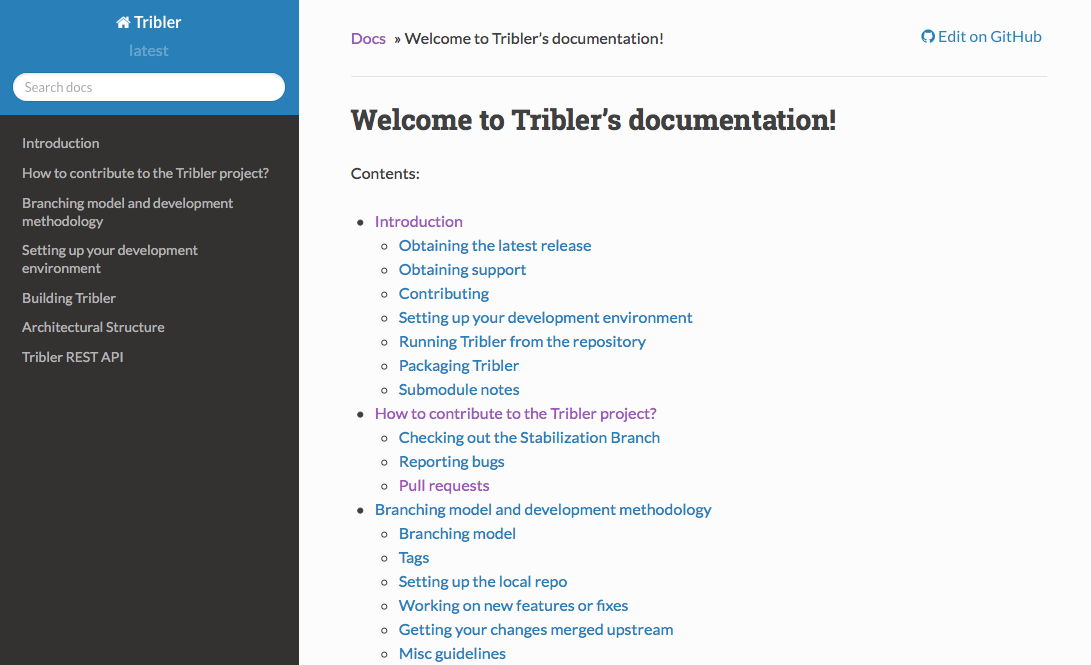
\includegraphics[width=1.0\columnwidth]{images/improving_qa/readthedocs}
	\caption{The new documentation base of Tribler, as available on the \emph{readthedocs} website.}
	\label{fig:old-threading-model}
\end{figure}

During this thesis, all available documentation of Tribler has been rewritten in RST format in conjunction with \emph{Sphinx}. Moreover, the available documentation has been expanded with several guides, in particular, guides that help new developers to set up an environment on their machine. Prior, these guides were not available and development on other platforms than Linux was not supported. By the addition of these guides, new developers can start as soon as possible with Tribler development.\\\\
The REST API in particular has been well documented. Since external developers should use the REST API to control Tribler, we wish to provide a clear and comprehensive documentation base for this API. To simplify the process of writing documentation, the documentation can be written as doc strings above each method in the source code. This documentation is parsed by the \emph{autosummary} tool that is executed each time the documentation is built: it navigates through the API code base, extracts all doc strings and generates separate sections for each annotated method. The doc string can be attributed with \emph{RST} syntax. This feature decreases chances that developers accidentally forget to write or update artifacts since the code and documentation is present in the same file instead of being spread across different distinct files.

\section{Preventing Technical Debt}
Prevention is the best medicine and we must think about a mechanism that prevents technical debt in future development stages. Developers have never been aware of the long-term consequences of the Tribler architecture and their work. To stop the deterioration of the system, we must raise awareness of technical debt and the term needs to play a more profound role when making long-term development decisions. To realise this, we present the following list of implemented ways to raise technical debt awareness:
\begin{itemize}
	\item Introducing mandatory code reviews of new PRs is an effective way of ensuring that problems in the code are detected as early as possible\cite{18fpreventdebt} but additionally, it helps developers to learn from their mistakes and to raise the quality bar of contributed code. The new policy introduced during this thesis requires each PR of developers to be reviewed by at least two other Tribler developers. This policy also helps developers to get more aware of ongoing work from other developers.
	\item Continuous integration and automated testing is an excellent opportunity to maintain a higher level of code quality and to catch bugs during the development process before end users are reporting them. The work as described in this Chapter, has matured the Jenkins and testing environment so it can be used reliably by the next generation of Tribler developers.
	\item Our CI environment already used static analysis tools to report violations in the source code which is an effective way to make developers aware of their introduced violations\cite{nagappan2005static}. However, when starting this thesis, these analysis tools have been implemented as separate jobs and were not executed on every pull request. This has been changed so developers receive fast feedback when they push a new commit to GitHub. The implemented checks executed for every PR are visible in Figure \ref{fig:jenkins-check}. Besides the reports of the test execution on multiple platforms and the code violation reporter, the code coverage report fails if developers added or modified lines that are not covered by a test. This tool will definitely contributes towards an increase of the code coverage metric in the long run.
\end{itemize}

\begin{figure}[h!]
	\centering
	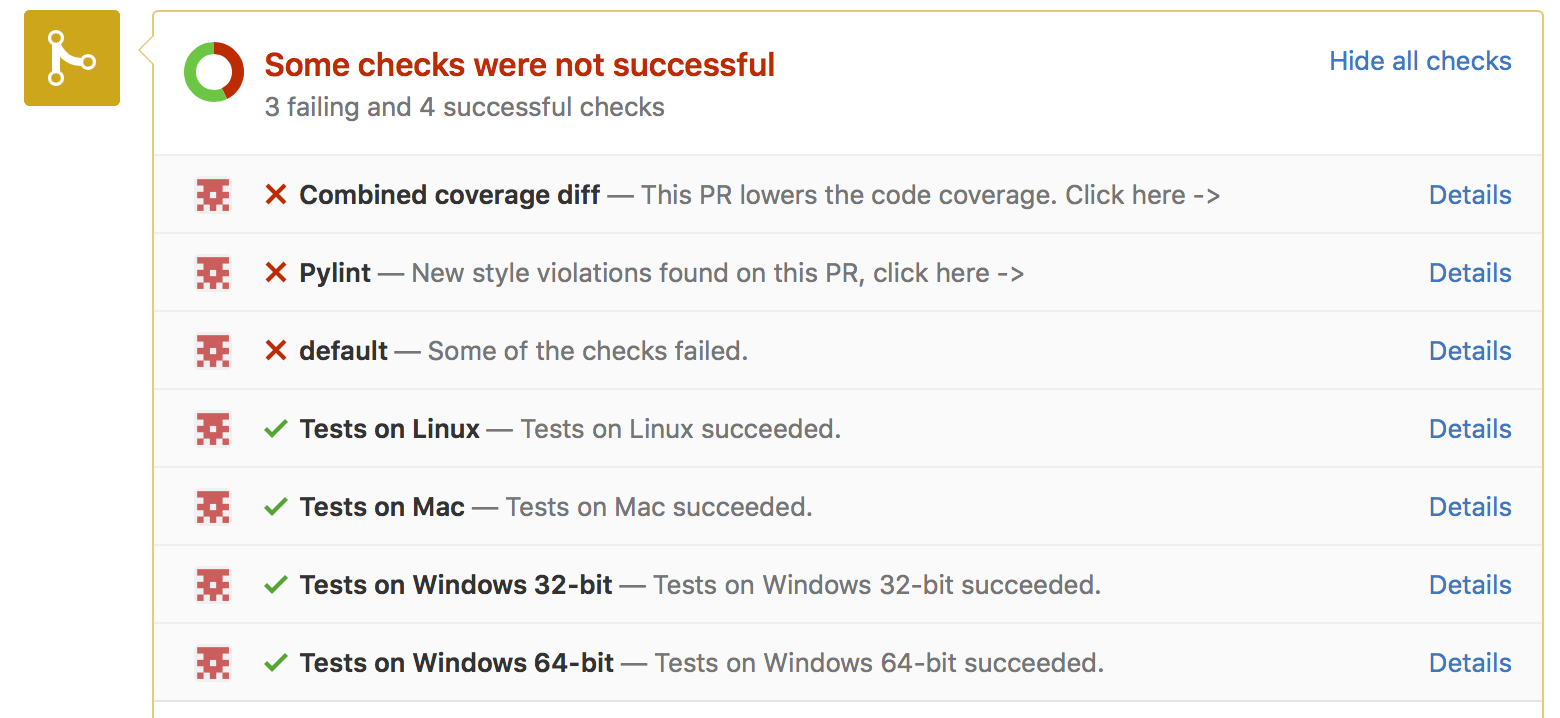
\includegraphics[width=1.0\columnwidth]{images/improving_qa/jenkins_checks}
	\caption{The implemented checks in Jenkins, executed on every new commit in a pull request.}
	\label{fig:jenkins-check}
\end{figure}